\section{Materiais Refratários Monolíticos}\label{mono}

	Os materiais refratários são componentes fundamentais nas economias modernas exercendo o papel de indústria habilitadora no sentido que possibilita a execução de processos a elevadas solicitações térmicas, químicas e mecânicas em um ambiente controlado e seguro. Ademais, o contexto sócio-ambiental do século XXI exige o máximo cuidado a fim de reduzir o desperdício de energia, especialmente de processos que ocorrem a altas temperaturas, onde a perda de energia para o ambiente é inerente.

	Assim, a indústria de materiais refratários está diretamente ligada a outras indústrias fundamentais como a indústria de cimento e principalmente a siderúrgica, ambas indústrias extremamente correlacionadas com o produto interno bruto (PIB) das nações, conforme demonstrado no gráfico temporal mostrado na Figura \ref{fig:refractory_economy}

\begin{figure}[ht]
\centering
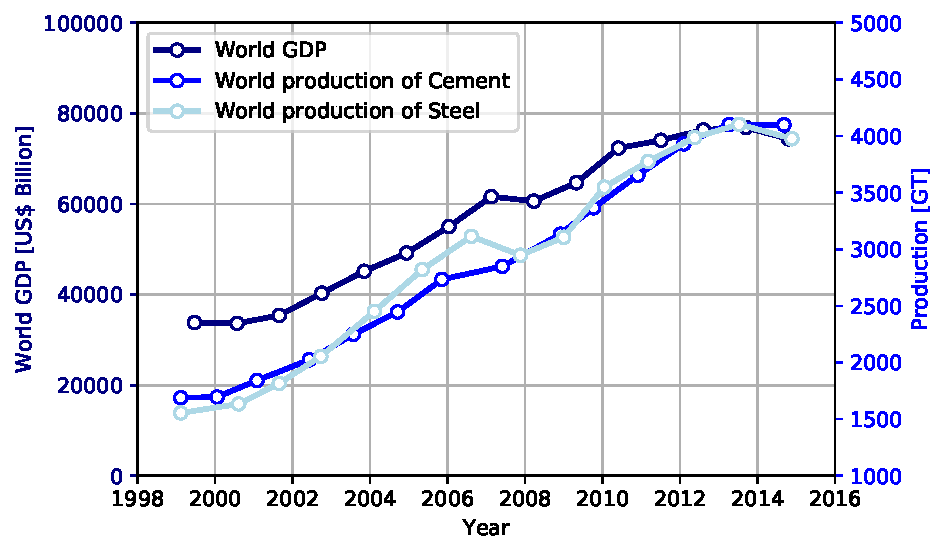
\includegraphics[width=\linewidth]{./figures/refractory_economy.pdf}
\caption{Evolução temporal do PIB mundial (azul escuro, eixo esquerdo), da produção mundial de Aço e Cimento (azul e azul claro, eixo direito) no período de 1999 a 2015.  Adaptado de \cite{GlobalRef2017}. \label{fig:refractory_economy}}
\end{figure}
		Com esse papel fundamental, os materiais refratários (que também passam por processos em alta temperatura durante sua fabricação) também passam por uma mudança de paradigma relativamente recente, isto é, ao invés do produtor fornecer peças pré-formadas (refratários conformados), este passa a oferecer um material conformável (monolítico), o que otimiza a logística - do ponto de vista do produtor, evita e reduz estoques, reduz o custo energético e permite uma maior customização do produto por parte do comprador.
        
        Dessarte, a seguir é realizada uma breve revisão do conceito de materiais monolíticos explorando seu processamento e finalmente vantagens e desvantagens características de tal classe de materiais.

    \subsection{Conceito}
    
    Dentro da classe de materiais monolíticos, a classe dos concretos ("\textit{castables}") é uma das que mais evoluíram recentemente. Uma motivação para sua evolução é sua facilidade de aplicação que aliada aos avanços em automatização gerou um interesse enorme no potencial dessa classe de materiais refratários, além de sua performance avançada \cite{Schacht2004}. Tal classe compreende materiais compostos, no geral, por agregados, uma matriz, ligantes, materiais secundários e aditivos o que amplia sua possibilidade de ajuste de propriedades.
    Os agregados formam o "esqueleto" do material, sendo os componentes de maior teor mássico dentro das formulações. A matriz é composta por materiais mais finos que objetivam maximizar o empacotamento do material, enquanto o ligante é o componente que confere a resistência mecânica de fato. Os materiais secundários são componentes mais baratos que também auxiliam na otimização do empacotamento da composição enquanto os aditivos são responsáveis a atribuir características que possibilitem os mais diversos tipos de metodologia de aplicação, como aceleradores e retardantes de pega, dispersantes e controladores de pH.
    A complexidade da formulação permite ajustes específicos que podem alterar as propriedades finais do produto. Um exemplo é o uso de agregados leves e porosos como uma maneira de redução da condutividade térmica, proporcionando um isolante com alta resistência mecânica, ou ainda o uso de carbono como um material secundário, que devido sua baixa molhabilidade por metais líquidos aumenta a resistência a corrosão do produto \cite{Schacht2004}.
    Outro fator importante da formulação, e que recentemente passou a definir inclusive quais as quantias de cada fração granulométrica, é o seu grau de empacotamento. Como resistência a ambientes altamente reativos é uma propriedade inerente dos materiais cerâmicos, a redução da porosidade foi uma das grandes motivações que levaram a consideração de teorias de empacotamento para o ajuste da formulação. Dentre as principais, listam-se a teoria de empacotamento de Alfred e o modelo de Andreasen \cite{Ortega1997}. 
    Tais avanços permitiram materiais cuja resistência mecânica obtida fosse relativamente elevada. Entretanto, um dos grandes contrapontos à maximização do empacotamento se dá na etapa de secagem do material. Especialmente em concretos com ligações hídricas (como sistemas com CAC), reações de desidratação passam a ocorrer na faixa de 210$\degree$C à 370$\degree$C, o que pode gerar vapores aprisionados na estrutura pouco permeável das composições de empacotamento otimizado, sendo possível que os níveis de pressão alcançados nessas regiões sejam maiores que a resistência mecânica do material levando à trincamento, lascamento e até mesmo explosões.
    
    \subsection{Processamento}
      O processamento de materiais refratários monolíticos é altamente dependente da metodologia de aplicação a ser utilizada.


    \subsection{Vantagens e desvantagens}
      Capítulos 10 e 11 - Livro Ana